\documentclass[11pt,letterpaper]{article}

% Load package
\usepackage{lesson}
\usepackage{amsmath}
\usepackage{xcolor}
\usepackage{url}

%--------------------------------------%
% Custom commands include:             %
%%%%%%%%%%%%%%%%%%%%%%%%%%%%%%%%%%%%%%%%
% Include an image:                    %
% \diagram{height}{align}{file}        %
%                                      %
% height: a number representing mm     %
% align: left, center, or right        %
% file: file name without extension    %
%%%%%%%%%%%%%%%%%%%%%%%%%%%%%%%%%%%%%%%%
% Add a numbered question:             %
% \question{text}                      %
% \questiond[lines]{file}{width}{text} %
%                                      %
% lines: # of lines of text to wrap    %
% file: file name without extension    %
% width: a % of textwidth for image    %
%%%%%%%%%%%%%%%%%%%%%%%%%%%%%%%%%%%%%%%%
% Add a lettered option/question part: %
% \option[vspace]{text}                %
%                                      %
% vspace: added space above the option %
%%%%%%%%%%%%%%%%%%%%%%%%%%%%%%%%%%%%%%%%
% Add a blank line in text:            %
% \blankline{width}                    %
%%%%%%%%%%%%%%%%%%%%%%%%%%%%%%%%%%%%%%%%
% Add an arc symbol in math:           %
% \arc{notation}                       %
%--------------------------------------%
%%%%%%%%%%%%%%%%%%%%%%%%%%%%%%%%%%%%%%%%
%--------------------------------------%
% To reset the question counter:       %
% \setcounter{qcounter}{0}             %
%                                      %
% To reset the option counter:         %
% \setcounter{acounter}{0}             %
%--------------------------------------%

% Set title and course name
\settitle{Week 4 Question Set}
\setsubtitle{Two-dimensional models and phase plane analysis \& Visual Brain}
\setcourse{Summer 2023}

\begin{document}

% Create title and add proper header for first page
\maketitle
\thispagestyle{first}

\section{CNS4.1 - From Hodgkin Huxley to 2D}
\begin{enumerate}
    \item \textbf{Reviewing the Hodgkin-Huxley Model}: Select the \textbf{incorrect} statement.
    \begin{enumerate}
        \item In the Hodgkin-Huxley Model, the time constant $\tau_x$ and the steady-state of the gating variable $x_0$ of a given ionic species $x$ are not actually constant, but depend on the voltage $u(t)$.
        \item The "battery" in the Hodgkin-Huxley model represents the passive process of ion diffusion down this established gradient, not the active process of pumping ions against the gradient.
        \item The gating variables in the Hodgkin-Huxley model exhibit an exponential decaying or saturating time course and have a tendency to return to their steady-state.
        \item The equilibrium potentials in the Hodgkin-Huxley model are determined by the relative permeabilities of the ion channels.
        \item The Hodgkin-Huxley model assumes that all ions have the same permeability at rest.
    \end{enumerate}

    \item \textbf{Separation of Timescales}: Consider a system of two differential equations: 
    \begin{align*}
        \frac{dx}{dt} & = -\frac{x - x_{0}}{\tau_x} + f(y) \\
        \frac{dy}{dt} & = -\frac{y - y_0}{\tau_y} + g(x)
    \end{align*}
    where $x$ and $y$ are the variables, $\tau_x$ and $\tau_y$ are their respective time constants, $x_0$ and $y_0$ are their steady-state values, and $f(y)$ and $g(x)$ are functions representing the influence of $y$ on $x$ and $x$ on $y$, respectively. 
    
    Assume that $\tau_x << \tau_y$, which means that $x$ reaches its steady state much faster than $y$ does. 
    
    \begin{enumerate}
        \item Under the assumption of separation of timescales, what does the first differential equation simplify to? What is the approximate steady-state value of $x$? 
        \vspace{2 cm}
        \item Using the steady-state value of $x$ obtained from the previous step, simplify the second differential equation. What does this equation look like? 
    \end{enumerate}
    \pagebreak

    \item \textbf{Simplifying System of Equations:} (This is a question from the lecture video) Often, systems of equations exhibit correlations or similarities that allow for simplification through substitution or combination. Consider two gating variables, $r$ and $s$, in a system. Under what conditions could we replace these with a single gating variable, $w$? Select the correct statement:
    \begin{enumerate}
    \item $r$ and $s$ have similar time constants as a function of $u$ and identical activation functions.
    \item $r$ and $s$ have similar time constants as a function of $u$ only.
    \item $r$ and $s$ have similar time constants as a function of $u$ and activation functions that are identical after some additive rescaling.
    \item $r$ and $s$ have similar time constants as a function of $u$ and activation functions that are identical after some multiplicative rescaling.
    \item $r$ and $s$ have identical activation functions only.
    \end{enumerate}
    \emph{Note}: Note, by activation function, I mean the differential equation that defines the dynamics of the gating variable, e.g. $dm / dt = -(m - m_0)/\tau_m$.

\end{enumerate}
\pagebreak

\section{CNS4.2 - Phase Plane Analysis}
\begin{enumerate}
    \item \textbf{Nullclines}: Understanding nullclines is crucial in the study of dynamical systems as they provide key insights into the system's behavior and stability. Consider the following system of equations which represents a model of interacting species, or a predator-prey model:

    \begin{align*}
        \frac{dx}{dt} &= x(1 - y) \quad \text{(1)} \\
        \frac{dy}{dt} &= y(x - 1) \quad \text{(2)}
    \end{align*}

    \begin{enumerate}
        \item A nullcline of a system of differential equations is defined as the set of points in the phase plane where the rate of change of a variable is zero. To find the nullclines for this system, we must separately set the right-hand side of each equation to zero and solve for the variables. Start by setting equation (1) to zero and solve for $y$ in terms of $x$. This will yield the nullcline for $x$. 

        \vspace{3 cm}

        \item Repeat the same process for equation (2), setting it to zero and solving for $x$ in terms of $y$. This will provide the nullcline for $y$.

        \vspace{3 cm}

        \item With the nullclines calculated, plot them on the phase plane. The intersection points of these nullclines will indicate the system's equilibrium points, which can provide valuable insights into the long-term behavior of the system.

        \pagebreak
    \end{enumerate}

    \item \textbf{Fixed points}: Consider a two-dimensional dynamical system with the following rate of change equations:
    \begin{align*}
    \frac{dx}{dt} &= x(1 - y) \\
    \frac{dy}{dt} &= y(x - 1)
    \end{align*}
    Which of the following statements is true about this system?
    \begin{enumerate}
        \item The fixed points are where either $x$ or $y$ is zero.
        \item The fixed points are the intersections of the nullclines, where the rates of change of both $x$ and $y$ are zero.
        \item All fixed points are stable; the system will always return to these points after a small perturbation.
        \item The system cannot have fixed points because both equations involve products of $x$ and $y$.
    \end{enumerate}

    \item \textbf{Flow Pattern}: Please sketch the vector field representing the dynamical system described above.

\end{enumerate}
\pagebreak

\section{CNS4.3 - Analysis of a 2D neuron model}
\begin{enumerate}
    \item \textbf{FitzHugh-Nagume Model with Pulse Current Input}: (This is a question from the lecture video) In a 2-dimensional neuron model, the effect of a \textbf{delta current pulse} can be analyzed. Select the correct option: 
    \begin{enumerate}
        \item By shifting the $u$-nullcline vertically upward, where $u$ represents the membrane potential.
        \item By shifting the $w$-nullcline vertically upward, where $w$ is a general gating variable.
        \item As a potential change in the stability or quantity of the fixed point(s).
        \item As a new initial condition.
        \item By following the trajectory in the appropriate phase plane according to the vector field.
    \end{enumerate}

    \item \textbf{FitzHugh-Nagume Model with Constant Current Input}: (This is a question from the lecture video) In a 2-dimensional neuron model, the effect of a \textbf{constant current input} can be analyzed. Select the correct option: 
    \begin{enumerate}
        \item By shifting the $u$-nullcline vertically upward, where $u$ represents the membrane potential.
        \item By shifting the $w$-nullcline vertically upward, where $w$ is a general gating variable.
        \item As a potential change in the stability or quantity of the fixed point(s).
        \item As a new initial condition.
        \item By following the trajectory in the appropriate phase plane according to the vector field.
    \end{enumerate}

    \item \textbf{FitzHugh-Nagumo Model Summary:} Select the correct option for each statement.
    \begin{enumerate}
        \item Using graphical analysis in the FitzHugh-Nagumo model, we can determine if a \textbf{pulse input} results in \underline{\hspace{2cm}} (action potential firing/repetitive firing).
        \item Similarly, we can determine if a \textbf{constant input} leads to \underline{\hspace{2cm}} (action potential firing/repetitive firing).
    \end{enumerate}

    \item \textbf{Limit cycle}: According to the simplified Poincaré–Bendixson theorem presented in the lecture, which of the following conditions can lead to the formation of a limit cycle? Select all that apply:
    \begin{enumerate}
        \item The system has one unstable fixed point.
        \item There exists a bounded region with only inward trajectories.
        \item The system displays chaotic behavior.
        \item There exists a bounded region with outward trajectories.
    \end{enumerate}

\end{enumerate}
\pagebreak

\section{CNS4.4A - Type I and Type II Neuron Models}
\begin{enumerate}
    \item Label the following figure as either Type 1 or Type II neuron:
    \begin{center}
        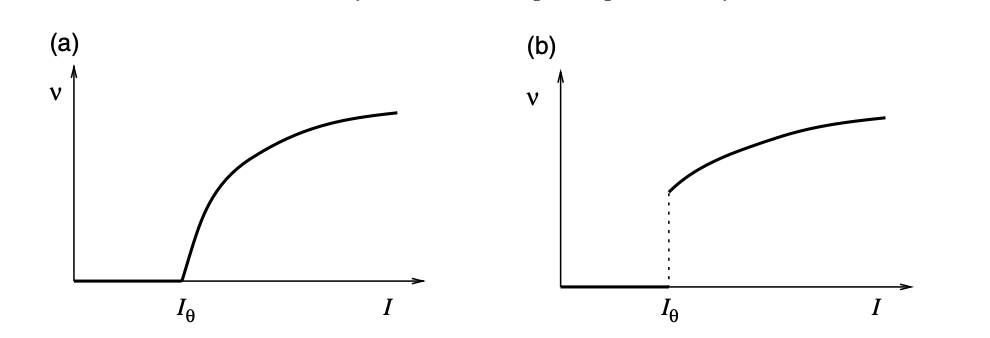
\includegraphics[scale=0.7]{4.1.png}
    \end{center}

    \item \textbf{Stability Analysis}: Arrange the following steps used in stability analysis of a 2D dynamical system in the correct order:
    \begin{enumerate}
        \item Put the first derivatives of the expansions into a matrix called the Jacobian matrix, which provides a linear approximation of the system dynamics near the equilibrium point.
        \item Perform a Taylor expansion of the system equations around the equilibrium point.
        \item Compute the eigenvalues of the Jacobian matrix. These eigenvalues give insight into the stability characteristics of the system near the equilibrium point.
        \item Determine the system's stability. If all the eigenvalues have negative real parts, then the equilibrium point is stable.
    \end{enumerate}
    \vspace{0.5 cm}
    Correct sequence: \underline{\hspace{6 cm}}
    \vspace{0.5 cm}

    \item \textbf{Hopf Bifurcation}: As discussed in the lecture, bifurcation refers to a change in the system's behavior as certain system parameters change. Specifically, a Hopf bifurcation occurs when a system's fixed point undergoes a change in its \underline{\hspace{2 cm}}, creating a limit cycle in the process. Choose the most appropriate option:
    \begin{enumerate}
        \item Position
        \item Dimensionality
        \item Shape
        \item Stability
    \end{enumerate}

    \item \textbf{Super- vs. Subcritical Hopf Bifurcations}: For each of the following scenarios, determine whether it most closely aligns with a supercritical ("super") or subcritical ("sub") Hopf bifurcation:
    \begin{enumerate}
        \item Type II neuron model, with a discontinuous frequency-current function. (sub/super)
        \item As a system parameter is varied, an initially stable equilibrium point loses its stability. Instead of the system becoming chaotic or unpredictable, a stable limit cycle emerges from the bifurcation point. (sub/super)
        \item As a system parameter is varied, an initially stable equilibrium point loses its stability, and an unstable limit cycle emerges, potentially leading to more complex or chaotic dynamics. (sub/super)
    \end{enumerate}
    

\end{enumerate}
\pagebreak

\section{CNS4.4B - Firing threshold in 2D models}
\begin{enumerate}
    \item \textbf{Saddle-Node Bifurcation}: Saddle-node bifurcation represents one of the fundamental types of bifurcations. In this process, a pair of fixed points, one stable and one unstable, are either created or annihilated. Identify the correct categorization for each fixed point during a saddle-node bifurcation:

    \begin{enumerate}
    \item The stable fixed point is termed as a: (Saddle/Node).
    \item The unstable fixed point is termed as a: (Saddle/Node).
    \end{enumerate}

    \item \textbf{Type I Model}: Considering the 2D Type I neuron model discussed in the video (prior to the bifurcation resulting in the loss of the saddle and node), what would be the neuron's response when the pulse input exceeds the threshold but is not sufficiently strong?
    \begin{enumerate}
        \item Delay in the initiation of the spike
        \item Decrease in the amplitude of the spike
    \end{enumerate}

    \item \textbf{FitzHugh-Nagume (Type II Model)}: Considering the 2D Type II neuron model discussed in the video, what would be the neuron's response when the pulse input is not sufficiently strong?
    \begin{enumerate}
        \item Delay in the initiation of the spike
        \item Decrease in the amplitude of the spike
    \end{enumerate}

    \item \textbf{Type I Model - Threshold}: In the context of the 2D neuron model showcased in the video, which of the following is responsible for determining the threshold of the action potential during saddle-node bifurcation with pulse input?
    \begin{enumerate}
        \item The stable manifold which attracts towards the saddle point.
        \item The u-nullcline which represents a set of points in the phase plane where the u-variable does not change.
        \item The w-nullcline which represents a set of points in the phase plane where the w-variable does not change.
    \end{enumerate}

    \item \textbf{FitzHugh-Nagume (Type II Model) - Threshold}: In the context of the 2D neuron model showcased in the video, which of the following is responsible for determining the threshold of the action potential under the assumption of the separation of timescales.
    \begin{enumerate}
        \item The stable manifold which attracts towards the saddle point.
        \item The middle branch of the u-nullcline.
        \item The middle branch of the w-nullcline.
    \end{enumerate}

\end{enumerate}
\pagebreak

\section{CNS4.5 - Nonlinear Integrate-and-Fire Model}
\begin{enumerate}
    \item \textbf{Further Reduction to 1D}: What does the separation of timescales enable us to accomplish? Select all that apply:
    \begin{enumerate}
        \item In the FitzHugh-Nagumo model, we can assume the slow variable $w$ to be constant. Therefore, in the phase portrait, the vector fields will be primarily horizontal except when near the u-nullcline.
        \item In the 2D Hodgkin-Huxley model, we can approximate $w$ to be constant near the resting state. This allows us to convert it into a 1D Exponential Integrate-and-Fire (EIF) Model with an exponential component and a linear subthreshold component. Since we are primarily interested in the timing of the spike and the subthreshold voltage, and not in modeling the adaptation and refractory period following the spike, we can introduce an explicit threshold and reset mechanism instead of having an additional variable $w$ after the spike.
    \end{enumerate}

\end{enumerate}
\pagebreak

\section{V\&B Chapter 4 - The Visual Brain}
\begin{enumerate}
    \item \textbf{Early Visual Pathway}: Arrange the components of the early visual pathway in their correct order of information processing. Write the corresponding letters in the correct sequence:
    \begin{enumerate}
        \item Primary visual cortex (V1), also known as the striate cortex
        \item Optic nerve
        \item Retinal ganglion cells
        \item Lateral geniculate nucleus (LGN)
        \item Optic chiasm
    \end{enumerate}
    Correct sequence: \underline{\hspace{6 cm}}

    \item \textbf{Optic Chiasm}: In creatures possessing eyes positioned on the sides of their heads, such as fishes, there is no crossing over of optic nerves. In these cases, visual information from each eye is relayed to the corresponding side of the brain. This setup offers an expansive field of view, which aids in identifying threats or potential meals.

    However, for species with eyes positioned towards the front, like many mammals, their visual fields show considerable overlap. In such scenarios, the optic chiasm plays a pivotal role by ensuring that visual input from the left field of view (from both eyes) is processed by the (left/right) brain hemisphere and the same applies for the right visual field. Choose the correct hemisphere to complete the sentence.

    \item \textbf{Lateral Geniculate Nucleus (LGN)}: The LGN is often characterized as a \underline{\hspace{2 cm}}, however it serves several other crucial functions. Which of the following best describes the primary function of the LGN?
    \begin{enumerate}
        \item A processor for auditory signals before they reach the auditory cortex
        \item A storage center for long-term visual memories
        \item A relay station for transmitting visual information from the retina to the visual cortex
        \item A generator of motor commands based on visual input
    \end{enumerate}

   \item \textbf{"M" and "P" Visual Streams}: The visual system segregates information into different processing streams, notably the Magnocellular ("M") and Parvocellular ("P") pathways. For each of the characteristics listed below, indicate whether it is primarily associated with the "M" or "P" pathway:
    \begin{enumerate}
        \item (M/P) Specializes in processing detailed information about color and form.
        \item (M/P) Excels in perceiving motion and spatial relationships.
        \item (M/P) Primarily mediates vision under low light conditions (scotopic vision) and is achromatic (lacks color sensitivity).
        \item (M/P) Predominantly mediates vision under well-lit conditions (photopic vision) and is chromatic (sensitive to color).
    \end{enumerate}

    \item \textbf{Simple and Complex Cells}: In their pioneering work, David Hubel and Torsten Wiesel identified two types of orientation-selective cells in the visual cortex: simple cells ("S") and complex cells ("C"). For each of the following characteristics, indicate whether it pertains to simple cells or complex cells:
    \begin{enumerate}
    \item (S/C) These cells have distinct excitatory and inhibitory subregions within their receptive fields.
    \item (S/C) These cells do not have distinct excitatory and inhibitory subregions; rather, they exhibit selectivity for certain features, such as line orientation.
    \item (S/C) These cells are selective for local features and their functional properties have inspired the design of convolutional layers in modern convolutional neural networks.
    \item (S/C) These cells aggregate the responses of other orientation-selective cells, providing the biological inspiration for the pooling layers in contemporary convolutional neural networks.
    \item (S/C) These cells are predominantly located in layers 2, 3, 5, and 6 of the primary visual cortex.
    \item (S/C) These cells are mainly found in the upper strata of layer 4 in the primary visual cortex.
    \end{enumerate}

    \item \textbf{The Packing Problem}: The brain's representation of different orientations, known as the "orientation map," features unique patterns called "pinwheels" (as seen in the figure below from Vidyasagar and Eysel, 2015, "Origins of feature selectivities and maps in the mammalian primary visual cortex").

    \begin{center}
    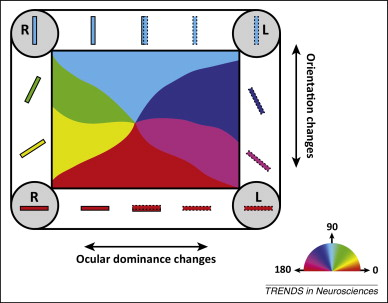
\includegraphics[scale=0.8]{pinwheel.jpg}
    \end{center}
    
    These pinwheels are a consequence of the brain's attempt to organize orientation preferences in a continuous fashion, from 0 to 180 degrees, onto a two-dimensional surface. Let's try a related problem. Given nine bars of different orientations (ranging from 0 to 180 degrees), can you arrange them in a $9 \times 9$ grid such that adjacent edges have similar orientations, and this pattern remains consistent when the grid is tiled (i.e., repeated across a larger surface)?
    \begin{center}
    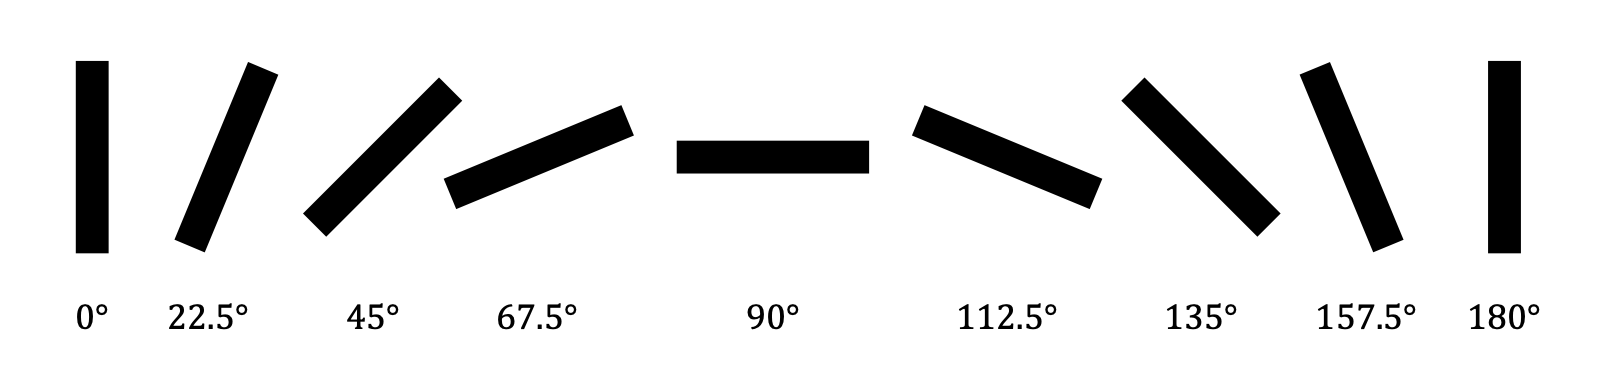
\includegraphics[scale=0.4]{orientations.png}
    \end{center}
    Is this task possible to achieve without creating "pinwheels"? Why or why not?
    
    
\includegraphics[scale=0.4]{grid.png}
    \pagebreak

    \item \textbf{Visual Areas}: For each description, choose the appropriate visual area from the following list: retina, LGN, V1, V2, V4, V5, and IT. Every area can only be used once.
    \begin{enumerate}
        \item \underline{\hspace{2 cm}}: The primary spatial organization principle seems to be viewpoint-centric. Also responds to high-level features such as faces.
        \item \underline{\hspace{2 cm}}: Identified by its stripy appearance. This area is rich in orientation-selective simple and complex cells as identified by Hubel and Wiesel. It features an organization pattern called "cortical columns" or "hypercolumns".
        \item \underline{\hspace{2 cm}}: Often referred to as the "motion" area due to its role in processing movement. Also responds to stereo disparity.
        \item \underline{\hspace{2 cm}}: Dubbed as the "relay station" of the visual pathway. There are two in the brain, each with six layers. Information from the left and right retinas alternate in complex sequences. This area also separates the magno- and parvocellular streams. Retains a retinotopic map.
        \item \underline{\hspace{2 cm}}: Contains photoreceptor cells which initiate the process of visual perception.
        \item \underline{\hspace{2 cm}}: Often referred to as the "color" cortex. This area also responds to simple shapes and objects. It primarily uses color and shape as its organizing principle, rather than strict retinotopic mapping.
        \item \underline{\hspace{2 cm}}: Characterized by three types of stripes. The thin stripes receive color blob inputs from V1, while the thick stripes receive input from orientation-selective (achromatic) neurons from V1.
    \end{enumerate}



\vspace{1 cm}


    

    
    
\end{enumerate}

\end{document}